\mychapter{TD1}
\label{Cap:TD1}


\section{Déscription physique}
Nous avons perçu que le système demandé sur la gestion d’une voie de péage d’autoroute.
%Nous avons élaborré dans ce document une première description de système d’un péage d’autoroute.

\begin{figure}[h]
    \centering
    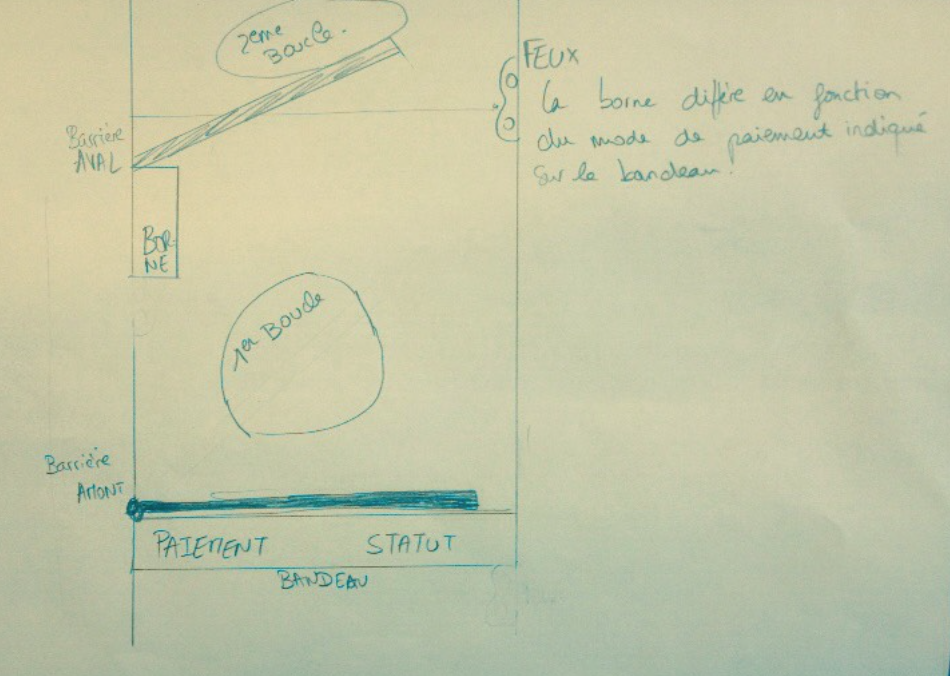
\includegraphics[scale=0.7]{images/a.png}
    \caption{Déscription physique}
    \label{fig:my_label}
\end{figure}
\newpage
\section{Réécriture de l'expression des besoins recentrée sur les utilisateurs du systeme}
\subsection{Les acteurs} 
Nous avons reconnu cinq acteurs  tel que :
\begin{itemize}
    \item \textbf{Le Client (conducteur de voiture)
}: Le conducteur est le client, le rôle du conducteur est de passer la barrière de péage autoroutiere. 
    \item \textbf{La Société d’autoroute}: 	La société est la propriétaire de la barrière de péage et gère donc la barrière. C’est lui qui va gérés aussi le carte d’abonnement et le traitement des comptes des abonnés. 
    \item \textbf{Le Technicien}: Le technicien sera le acteur premiere pour la maintenance du système.  
    \item \textbf{Operateur}: Il va superviser l’ensemble des bornes, pour assurer, par exemple, que à tout moment il y a une voie ouverte ou que le nombre de voies ouvertes sont proportionnel au flux de véhicules. Il va faire une intervention si le système lever une alarme vers l’ordinateur du poste de surveillance pour que le operateur pratique un rendu “approximatif” si necessaire.
\end{itemize}

\subsection{Fonctionnalités}
Nous avons différencié trois fonctionnalités :
\textbf{Passer le péage }(\ref{subsubsec:passerL})

\textbf{Gerer la comptapilité
} (\ref{subsubsec:gerer})

\textbf{Maintenance}(\ref{subsubsec:maint})

Ainsi voici les scénarios informels correspondant :
\subsubsection{\textbf{Cas d’utilisation:} Passer le péage } \label{subsubsec:passerL}
\textbf{Acteur primaire}: Le Client (le conducteur)\\

\textbf{Acteur support}: L’operateur et La Société d'autoroute.\\

Selon son type de véhicule, et le moyen de paiement qu’il préfère, le conducteur va se diriger vers la voie la plus adapté. Il se dirigera vers une voie ouverte et pourra choisir son mode de paiement grâce à la gestion d’ouverture des voies.
Le passage d’un conducteur entraine un paiement en fonction du type de véhicule et déclenche le système d’ouverture des barrières.


\subsubsection{\textbf{Cas d’utilisation:} Gerer la comptabilité}  \label{subsubsec:gerer}
\textbf{Acteur primaire}: La Société d'autoroute \\

Après paiement du client les données sont transmises à la société déclenchant les mécanismes de comptabilité. Après passages des abonnés, la société d’autoroute va engendrer les mécanismes associés

\subsubsection{\textbf{Cas d’utilisation:} Maintenance}  \label{subsubsec:maint}
\textbf{Acteur primaire}: Le Technicien  
